\section{AMIDST model class}

\textcolor{red}{OUt-of-topic: Shouldn't we use Figure numbering based on section? The deliverable is expanding like the universe...}\\
One of the main goals of AMIDST project is the definition of a general model class with the following characteristics: 

\begin{itemize}
\item It should be applicable to the three considered use-cases, i.e., Daimler, Cajamar, and Verdande,

\item it should be scalable, supporting both inference and learning from massive data streams.

\item it should be general enough to be applicable to any future, potentially similar, use-cases, and

\end{itemize}

Taking these different characteristics into account, and using the subnetwork graphical notation (see Section \ref{Section:Preliminaries}), we will first present and discuss the general AMIDST model class in Section \ref{GeneralModelClass}, then its specific instantiation to each use-case in Section \ref{UseCaseModelClasses}.

%---------------------------------------------------------------------
\subsection{The general AMIDST model class}\label{GeneralModelClass}
%---------------------------------------------------------------------

Figure \ref{Figure:AMIDSTModelClass} shows the proposed general AMIDST model class. This model is the result of combining all the models required by the different problem domains above presented. In order to find the commonalities between all models, higher-level descriptors have been required to reinterpret the individual models, that is, instead of all the individual variables, subnetworks have been used to group variables with similar properties.


\begin{figure}[ht!]
\begin{center}
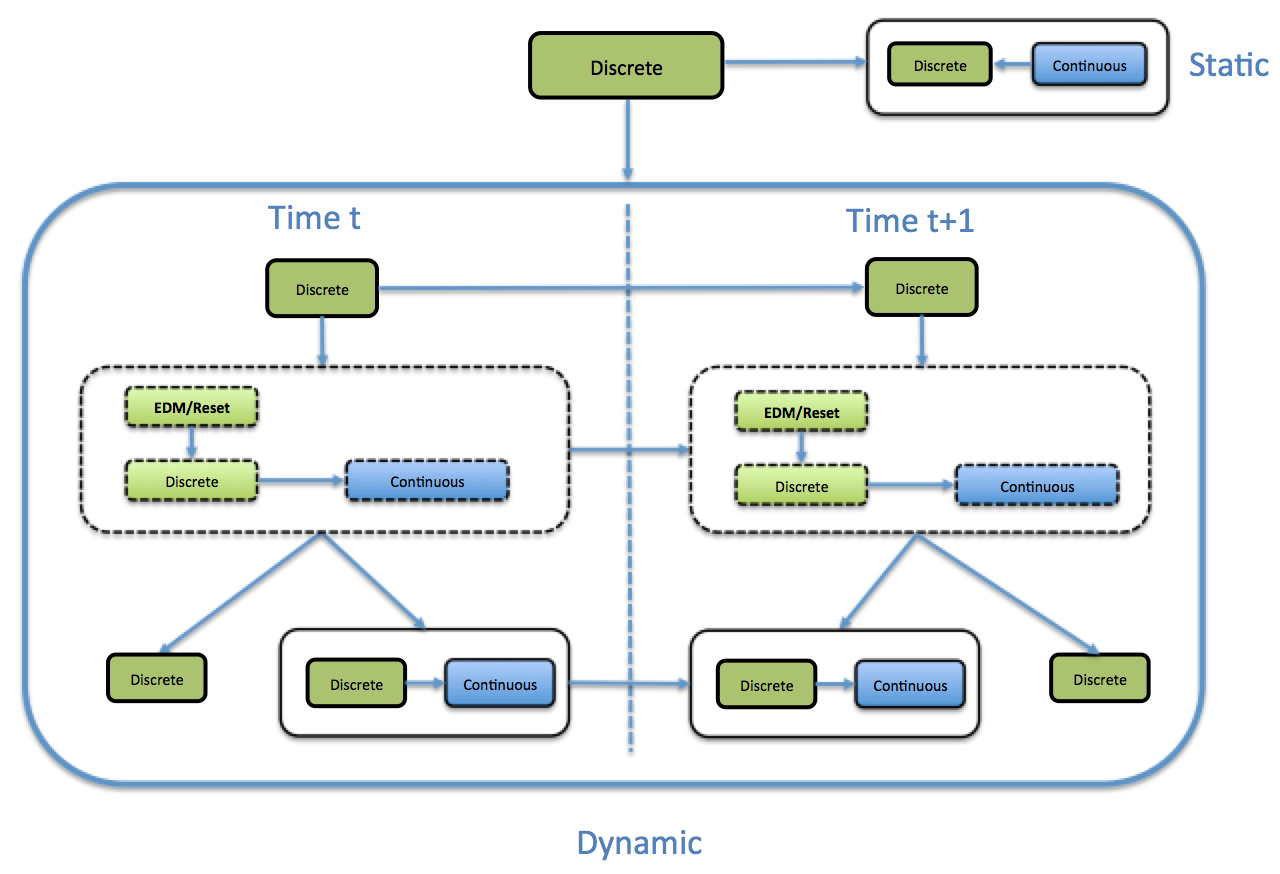
\includegraphics[scale=0.39]{./figures/AMIDSTModelClass}
\caption{\label{Figure:AMIDSTModelClass} Proposed AMIDST model class.}
\end{center}
\end{figure}


Although the resulting model might not be very revealing at the moment, we can indeed distinguish 3 different layers. The upper layer corresponds to the continuous observed variable, namely ``Continuous 1", and we will refer to it as \textit{input layer}. The second layer corresponds to a set of interconnected discrete and continuous variables, for which only links from discrete to continuous nodes are allowed. We will refer to it as the \textit{state layer}. Finally, the bottom layer corresponds to a set of interconnected discrete and continuous observed variables, in which in principles, there exist no restrictions with respect to the direction of the links, although only links from discrete to continuous nodes are required by our use cases. This layer will be referred to as \textit{output layer}. A representation of this higher level of abstraction is shown in Figure \ref{Figure:AMIDSTModelClassHighLevel}. \textcolor{red}{Add layer names to Figure \ref{Figure:AMIDSTModelClassHighLevel}}

\begin{figure}[ht!]
\begin{center}
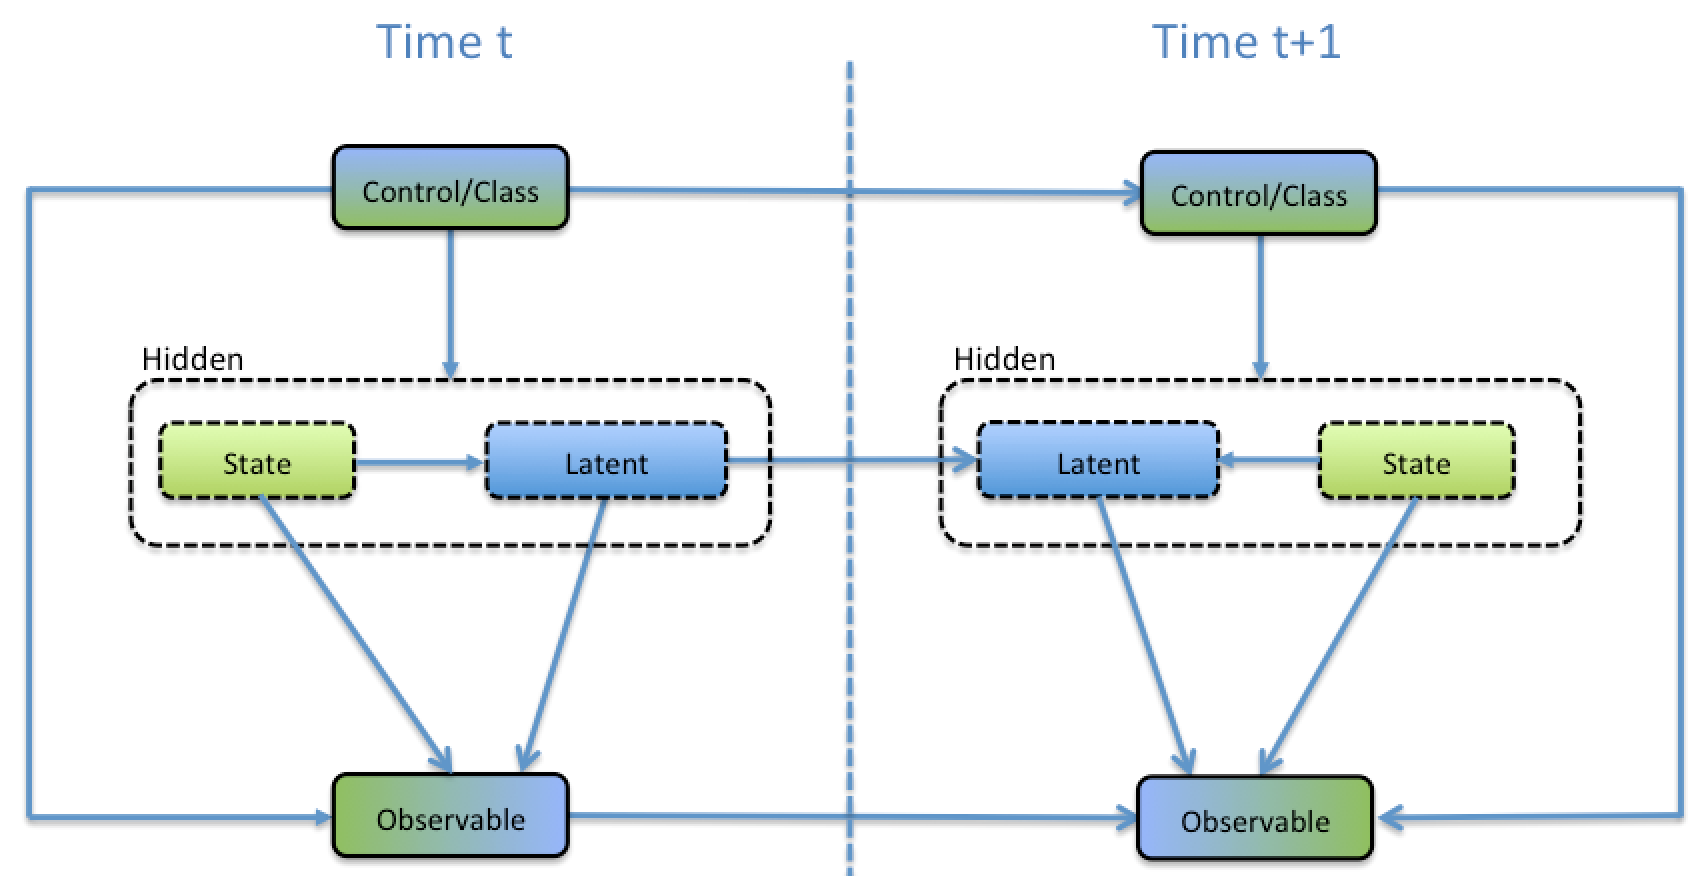
\includegraphics[scale=0.4]{./figures/AMIDSTModelClassGeneral}
\caption{\label{Figure:AMIDSTModelClassHighLevel} The high-level AMIDST model class}
\end{center}
\end{figure}

In the following sections, we will reason out how each particular use case fits in this global model.

%---------------------------------------------------------------------
\subsection{The model classes of the three use-cases} \label{UseCaseModelClasses}
%---------------------------------------------------------------------

In the following section, we will re-introduce the model classes of the three use-cases (that have been previously presented in Section \ref{Section:PreliminaryModels}) but using a higher level of abstraction. 

%---------------------------------------------------------------------
\subsubsection{Daimler model class}\label{daimlerAMIDSTModels}
%---------------------------------------------------------------------

\textcolor{blue}{To be re-written}
Daimler's models have been previously described in Figures \ref{Figure:daimlerLEdynGeneric} and \ref{Figure:daimlerreldyn}. As commented in Section \ref{Section:DaimlerDynamic}, one the main issues of these current models is that they contain discrete children with continuous parents, and do not fall into the conditional linear Gaussian family \cite{JensenNielsen2007}. To deal with this problem, we adopt here the same solution pursed in \cite{kasper2012object} which consists in discretizing these nodes. In this way, the general structure of Daimler's models corresponds to the one depicted in Figure \ref{Figure:DaimlerModelClass}, where there is no more discrete children with continuous parents, and it is possible thereby to use standard parametrizations \cite{JensenNielsen2007}. 


\begin{figure}[ht!]
\begin{center}
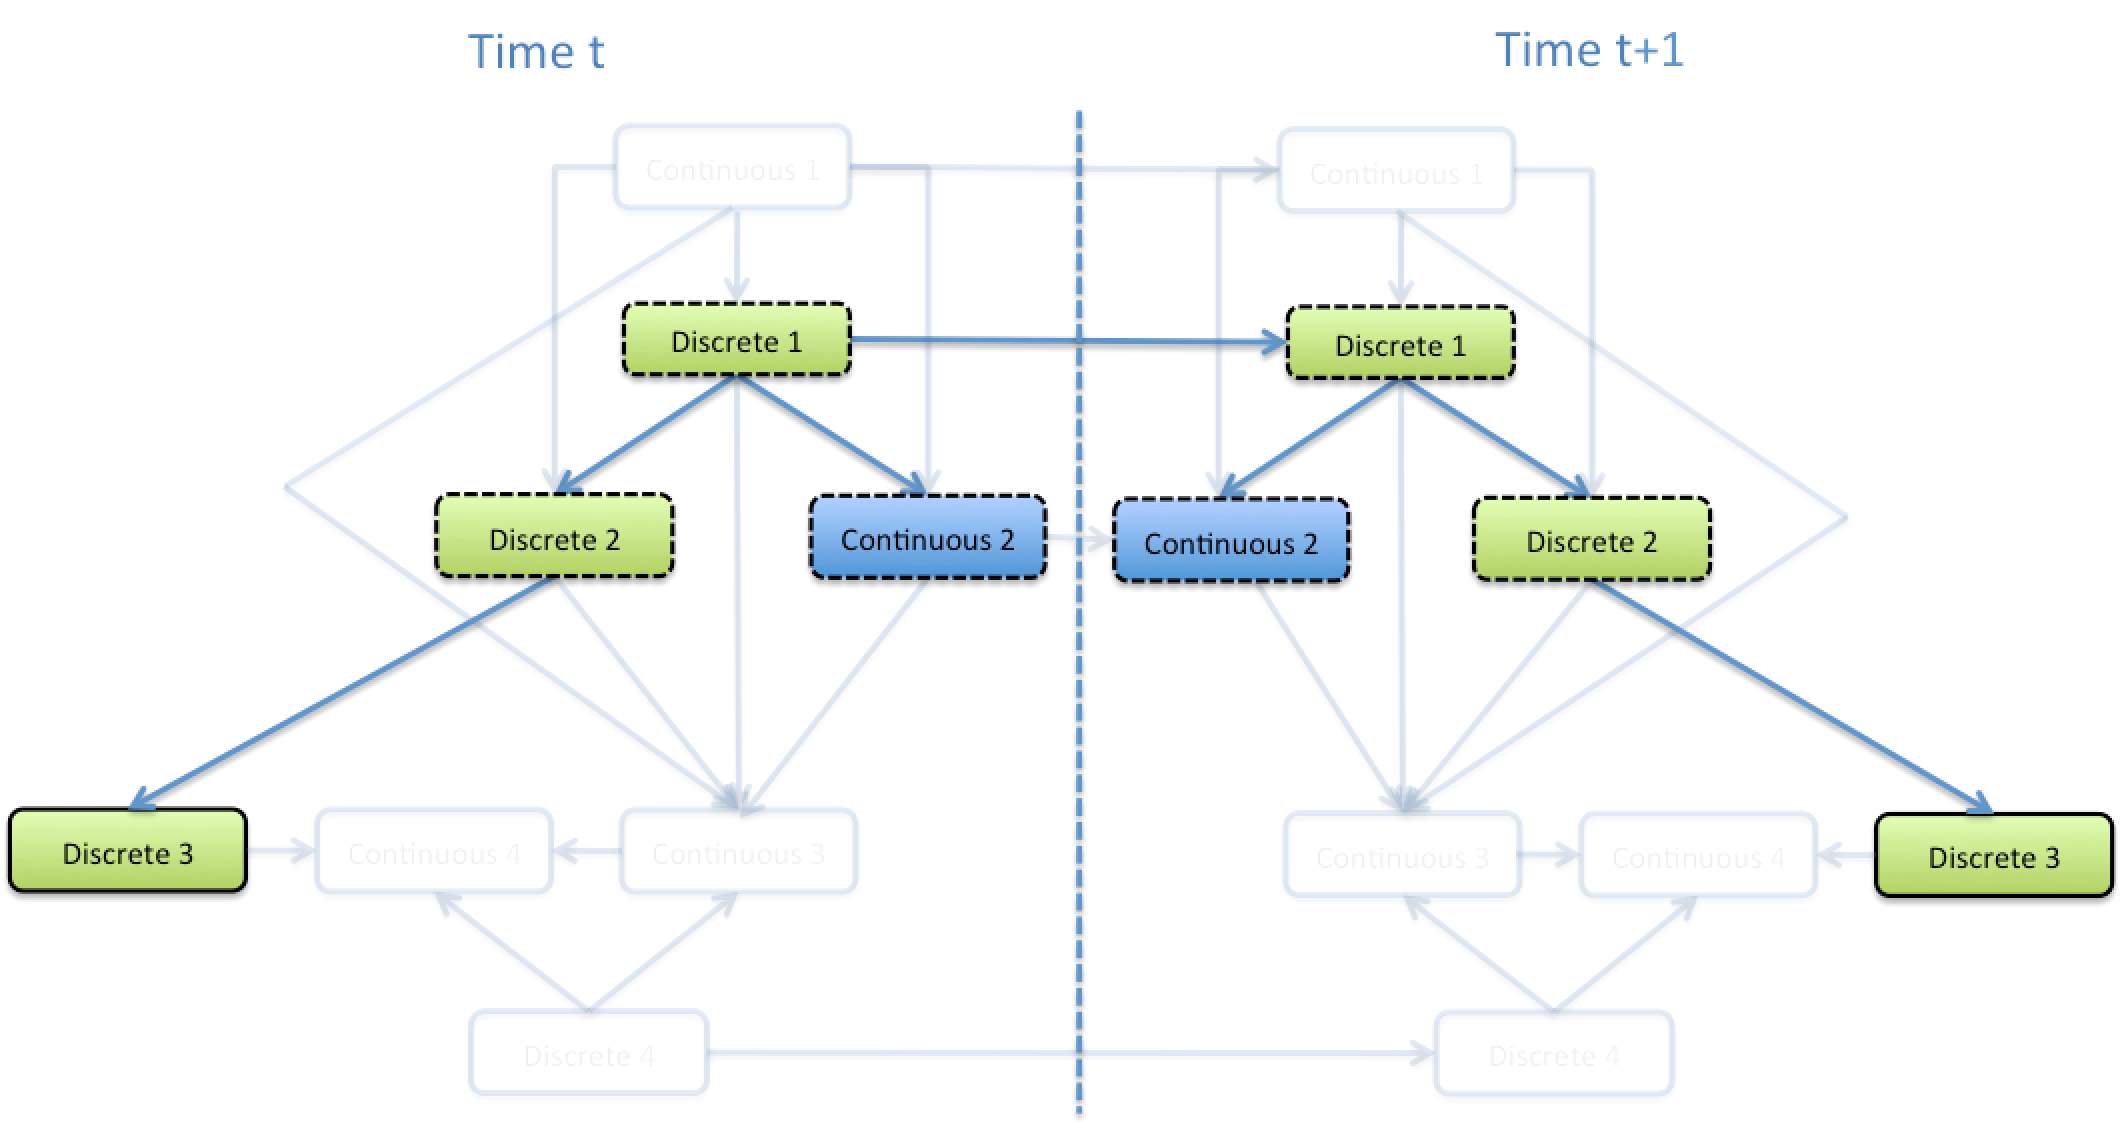
\includegraphics[scale=0.39]{./figures/AMIDSTModelClassDaimler}
\caption{\label{Figure:AMIDSTModelClassDaimler} AMIDST model class - Daimler}
\end{center}
\end{figure}

%\begin{figure}[ht!]
%\begin{center}
%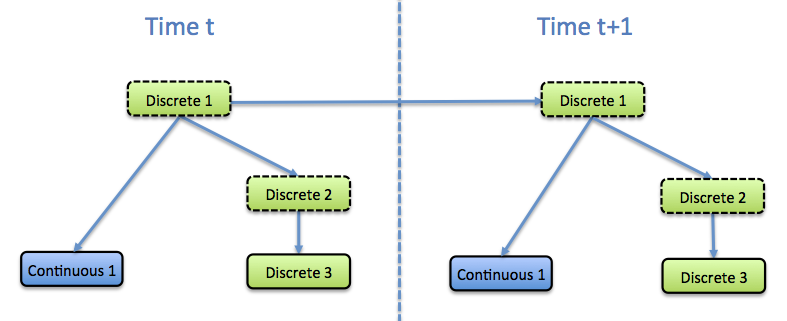
\includegraphics[scale=0.4]{./figures/DaimlerModelClass}
%\caption{\label{Figure:DaimlerModelClass} Daimler model class}
%\end{center}
%\end{figure}

This general model is structured as a 2T-DBN (see Section \ref{SubSubSection:2DBNs}). The static model which is repeated over time consists of four elements: 

\begin{enumerate}
\item ``Discrete 1'': is a discrete hidden subnetwork which is the only element temporally connected
\item ``Discrete 2'': is an additional discrete hidden subnetwork which is not temporally connected. It is included only for modelling purposes inside a time slice
\item ``Discrete 3'': is an observed discrete subnetwork directly depending on ``Discrete 2'' subnetwork
\item  ``Continuous 1'': is an observed continuous subnetwork which is directly depending on ``Discrete 1'' subnetwork
\end{enumerate}

As commented, this 2T-DBN is only temporally connected through the hidden subnetwork on top. Consequently, the future and past time slices of our 2T-DBN are conditionally independent given the hidden subnetwork corresponding to the present time. Additionally, inside a time slice, the observed continuous and discrete subnetworks are also conditionally independent given this hidden subnetwork.

In addition, we have more structure that can be exploited during inference and which is not reflected in this meta-network. Specifically, the hidden and observed subnetworks may have a polytree structure \cite{JensenNielsen2007}. In this case, both static and dynamic BNs have polytree structure and this can be exploited during inference. 

%---------------------------------------------------------------------
\subsubsection{CajaMar model class}
%---------------------------------------------------------------------
\textcolor{blue}{To be re-written}
Concerning CajaMar use-case, both application scenarios share the same models, of which two versions have been previously discussed, namely, static and dynamic (see Section \ref{Section:CajaMarModels}). 

At this point, we obviate the static version, because the general AMIDST model class is primarily a dynamic model class. Therefore, the high-level description of CajaMar's dynamic model is given in Figure \ref{Figure:CajaMarModelClass}. As it can be seen, CajaMar models is composed by four main subnetworks, which are expanded over time and all of them are observed. Hence, at CajaMar, there are no hidden subnetworks. 


\begin{figure}[ht!]
\begin{center}
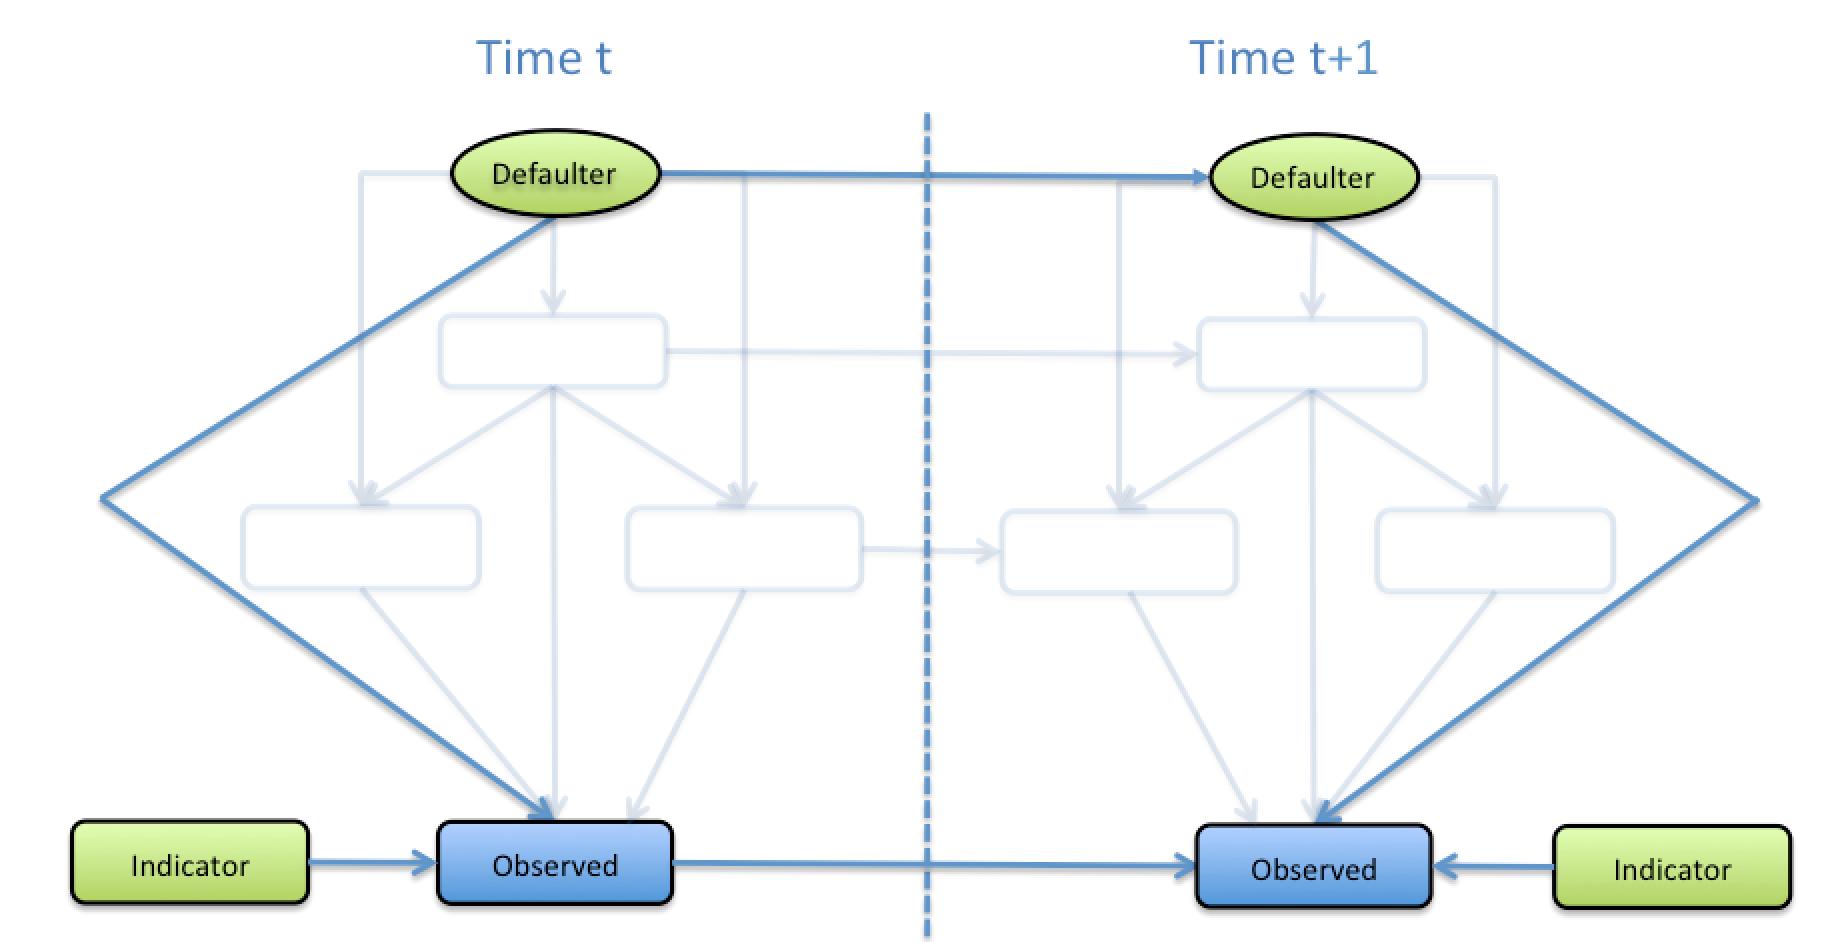
\includegraphics[scale=0.39]{./figures/AMIDSTModelClassCajamar.png}
\caption{\label{Figure:AMIDSTModelClassCajamar} AMIDST model class - Cajamar.}
\end{center}
\end{figure}

%\begin{figure}[ht!]
%\begin{center}
%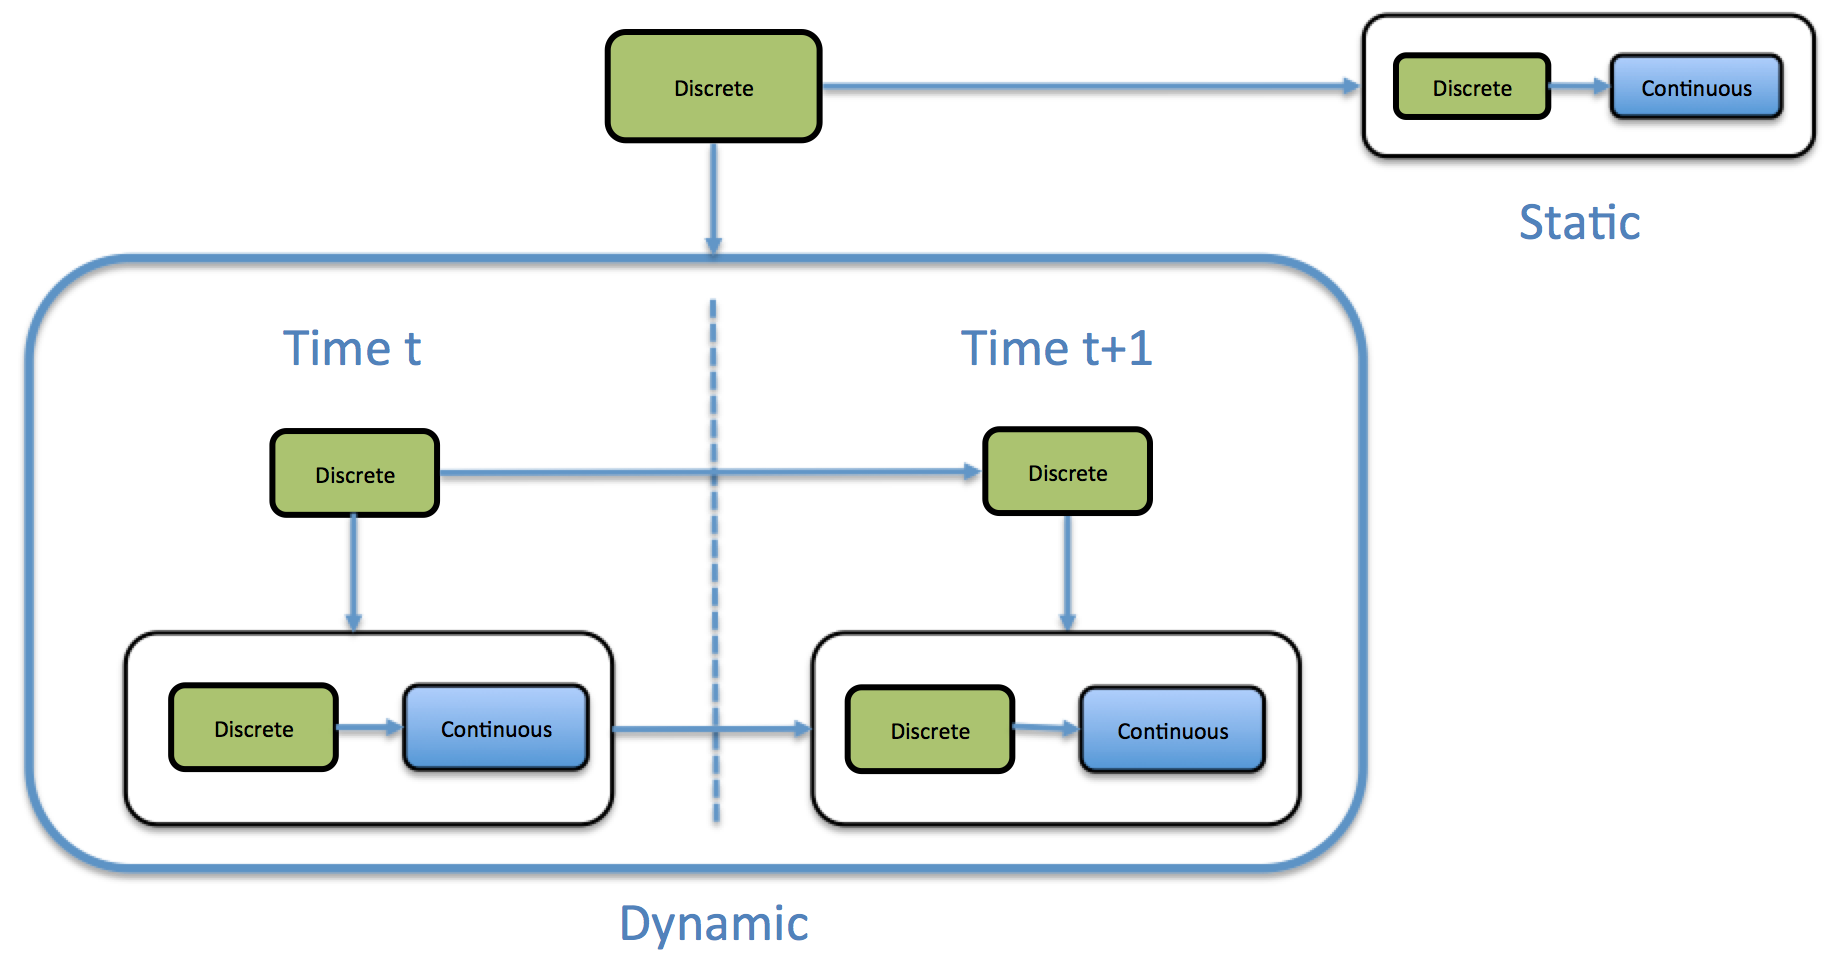
\includegraphics[scale=0.4]{./figures/CajaMarModelClass}
%\caption{\label{Figure:CajaMarModelClass} CajaMar model class}
%\end{center}
%\end{figure}

%---------------------------------------------------------------------
\subsubsection{Verdande model class}
%---------------------------------------------------------------------
\textcolor{blue}{To be re-written}
Verdande's models were visually described in Figures ?, ? and ? for the three identified application scenarios (see Section \ref{Section:VerdandeModels}). Figure \ref{Figure:VerdandeModelClass} visually depicts the high-level model class that subsumes the different models of the three application scenarios. As it can be seen, it is possible to distinguish three interpretations each corresponding to an application scenario:

\begin{itemize}
\item If we keep the subnetworks ``Discrete 2'', ``Continuous 1'' and ``Continuous 2'', we obtain the switching Kalman filter model for application scenario 1 (see Section \ref{SubSection:DetectionTorque}),
\item If we keep ``Continuous 1'', ``Discrete 3'' and ``Continuous 2'', we obtain the input-output Kalman filter model for application scenario 2 (see Section \ref{SubSection:SemiAutomaticLabelling}), and
\item finally, if we keep ``Discrete 1'', ``Discrete 2'' and ``Continuous 2'', we obtain the input-output Kalman filter model for application scenario 3  (see Section \ref{SubSection:DetectionFormation}).
\end{itemize}



\begin{figure}[ht!]
\begin{center}
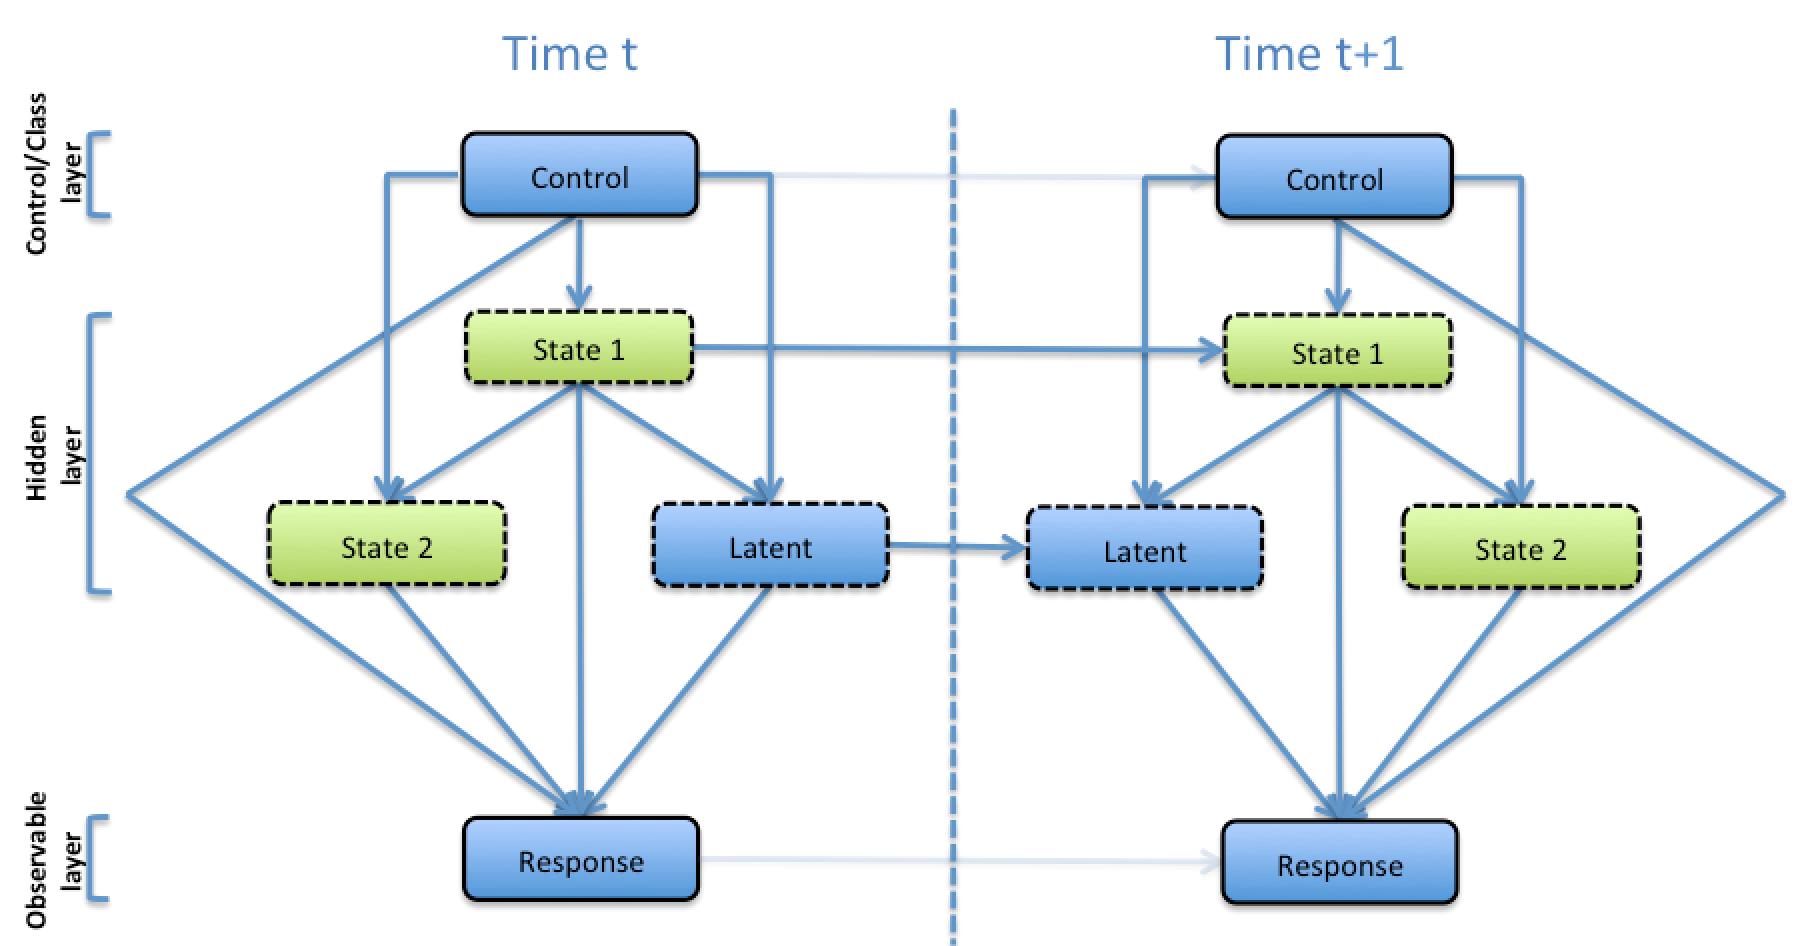
\includegraphics[scale=0.39]{./figures/AMIDSTModelClassVerdande}
\caption{\label{Figure:AMIDSTModelClassVerdande} AMIDST model class - Verdande.}
\end{center}
\end{figure}

%\begin{figure}[ht!]
%\begin{center}
%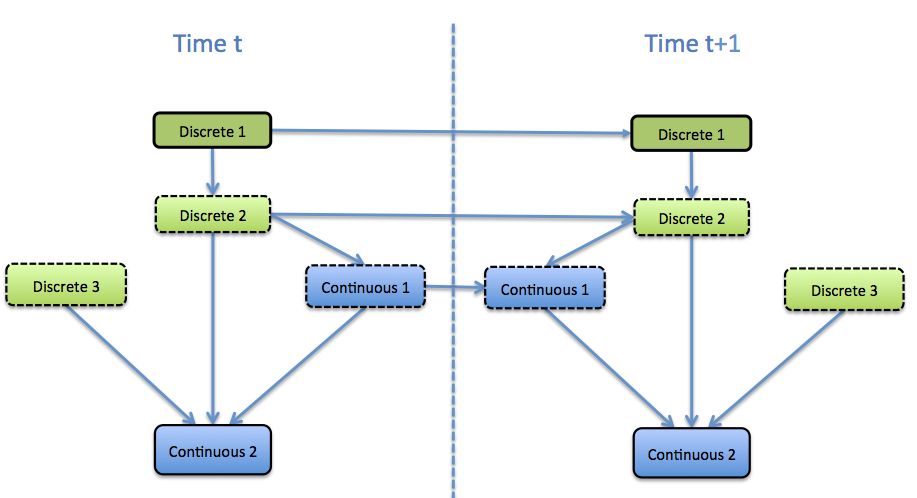
\includegraphics[scale=0.4]{./figures/VerdandeModelClass}
%\caption{\label{Figure:VerdandeModelClass} Verdande model class}
%\end{center}
%\end{figure}

Similarly to the Daimler model, the general model is structured as a 2T-DBN (see Section \ref{SubSubSection:2DBNs}). The static part which is repeated over time is composed by five subnetworks: two observed components (i.e., one discrete temporally connected on the top, and one continuous at the bottom); and three hidden components in the middle (i.e., one hidden discrete and one hidden continuous both are temporally connected, and one hidden discrete, which is not temporally connected and its function is to account for the possible conditional dependencies of the observed continuous variables).  

However, contrary to Daimler, Verdande class model does not have a polytree structure that can be exploited during inference. 


\subsection{Summary}

%This section, with the high-level figure, should help to defend the third point made in the introduction, i.e., that it should be general enough to be applicable to any future, potentially similar, use-cases.
 


%\begin{figure}[ht!]
%\begin{center}
%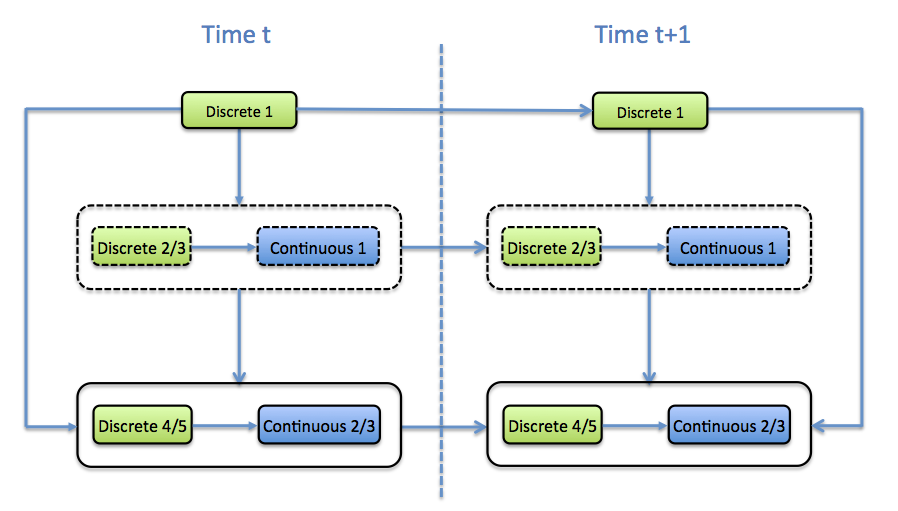
\includegraphics[scale=0.4]{./figures/AMIDSTModelClassHighLevel}
%\caption{\label{Figure:AMIDSTModelClassHighLevel} AMIDST model class high level}
%\end{center}
%\end{figure}

%\begin{figure}[ht!]
%\begin{center}
%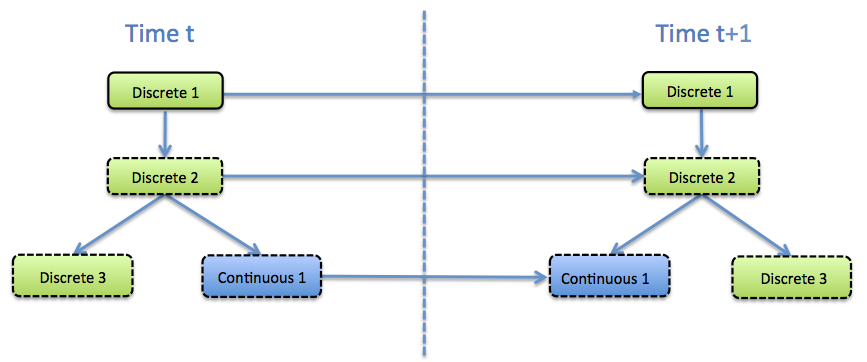
\includegraphics[scale=0.4]{./figures/AMIDSTModelClassTopPart}
%\caption{\label{Figure:AMIDSTModelClassHighLevel} AMIDST model class top part}
%\end{center}
%\end{figure}
%
%\begin{figure}[ht!]
%\begin{center}
%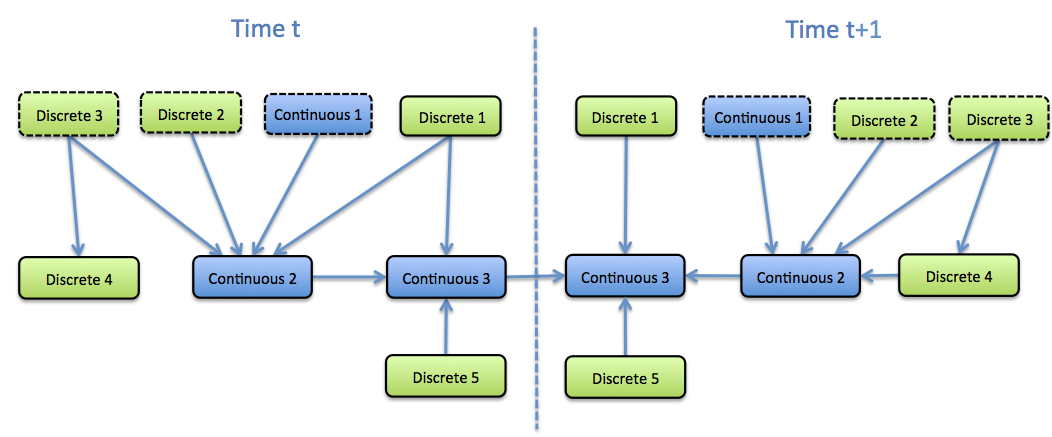
\includegraphics[scale=0.4]{./figures/AMIDSTModelClassLowPart}
%\caption{\label{Figure:AMIDSTModelClassHighLevel} AMIDST model class low part}
%\end{center}
%\end{figure}